\appendix
\chapter{Null space inverse kinematics}
\label{apx:null-space}
As discussed in \refsec{sec:trajectories}, inverse kinematics will be an underdetermined system if the number of controllable joints exceeds the degrees of freedom of the desired end effector pose. This has the effect of having infinitely many, all equally valid robot poses which achieve the desired end effector position. However, this is only in theory. Consider \reffig{fig:ik-invalid}. Here we can see that the solution requires two of the arm links to intersect. While this is fine in theory and does constitute a solution to the IK system, in the real world the links of the robot arm are not infinitely thin line segments, they are physical parts with thickness. If this robot was in the real world this would require parts of the robot to pass through each other. This is obviously impossible in a real situation.

\begin{figure}[h]
    \centering
    \begin{subfigure}[b]{0.45\textwidth}
        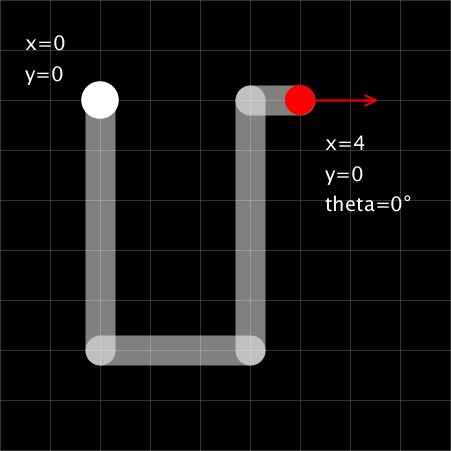
\includegraphics[width=\textwidth]{figures/ik-valid.png}
        \caption{A valid IK solution}
        \label{fig:ik-valid}
    \end{subfigure}
    \hfill
    \begin{subfigure}[b]{0.45\textwidth}
        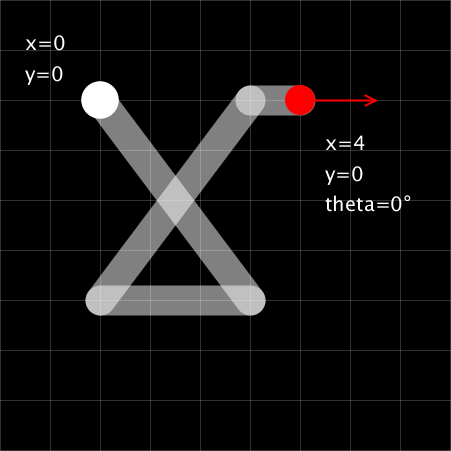
\includegraphics[width=\textwidth]{figures/ik-invalid.png}
        \caption{An invalid IK solution}
        \label{fig:ik-invalid}
    \end{subfigure}
    \caption{Not all IK solutions may be valid}
    \label{fig:ik-null-space}
\end{figure}

Fortunately for us, we saw that by having additional degrees of freedom, we can generate infinitely many solutions to the IK system. This means we could prune these invalid solutions by adding additional constraints. While it is possible this could make all solutions invalid, this is both unlikely and necessary. These invalid solutions remain because the current IK system does not perfectly capture our real world restrictions. If all solutions are removed by our additional constraints, then this simply means the desired end effector pose was not possible in a real world system.\\

There are two main ...



\chapter{Evaluation Test Suite}
\label{apx:test-suite}

This appendix details specifics about the test suite used in \refchap{chap:evaluation}.\\

\begin{figure}[h]
    \centering
    \begin{subfigure}[b]{0.49\textwidth}
        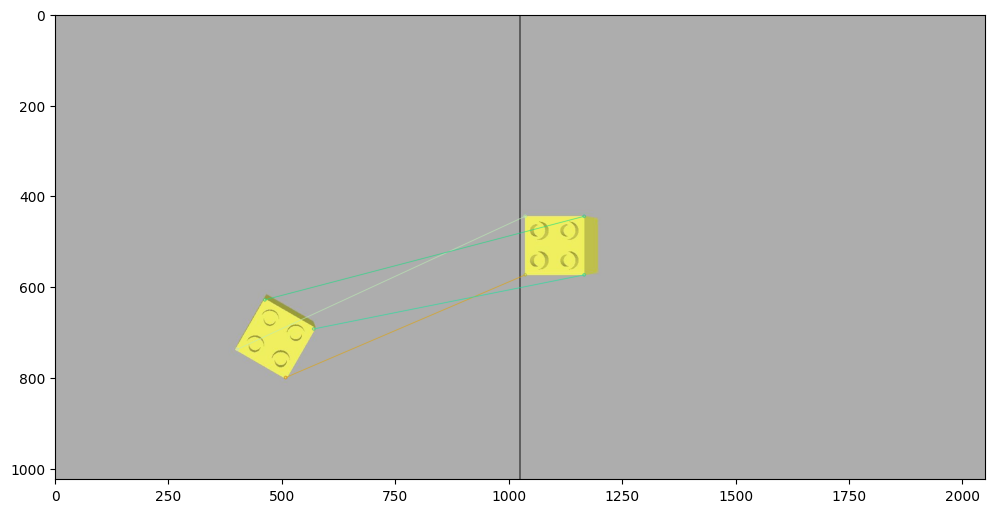
\includegraphics[width=\textwidth]{figures/matchLego.png}
        \caption{Lego object}
    \end{subfigure}
    \hfill
    \begin{subfigure}[b]{0.49\textwidth}
        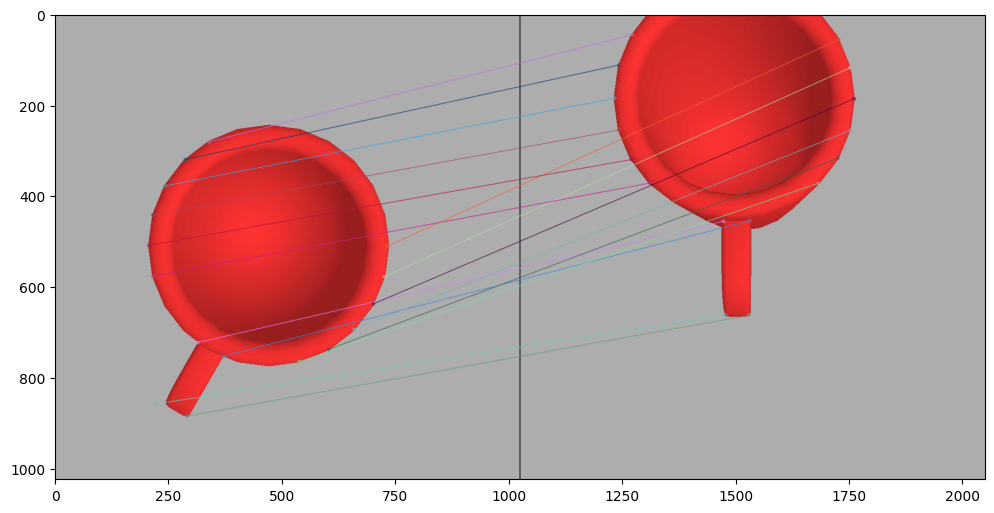
\includegraphics[width=\textwidth]{figures/matchMug.png}
        \caption{Mug object}
    \end{subfigure}

    \begin{subfigure}[b]{0.49\textwidth}
        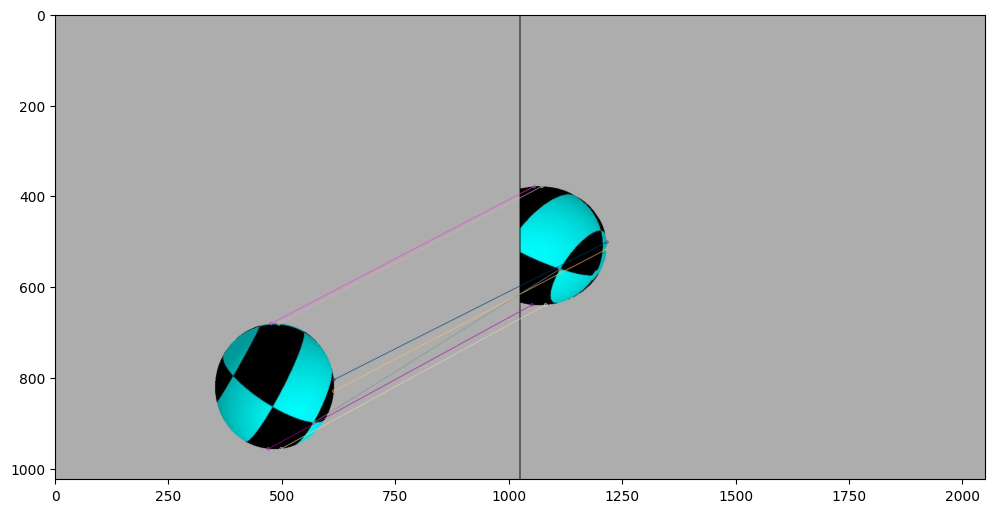
\includegraphics[width=\textwidth]{figures/matchBall.png}
        \caption{Ball object}
    \end{subfigure}
    \hfill
    \begin{subfigure}[b]{0.49\textwidth}
        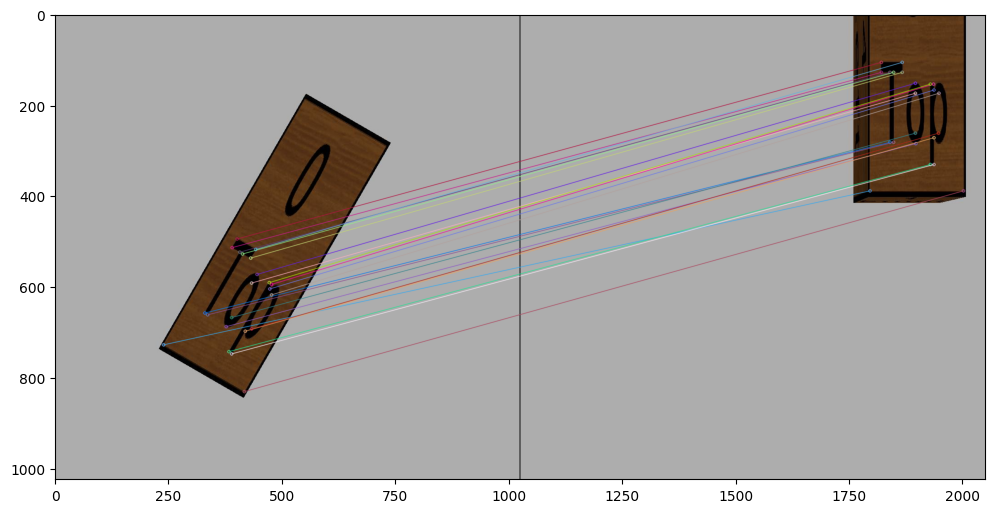
\includegraphics[width=\textwidth]{figures/matchJenga.png}
        \caption{Jenga block object}
    \end{subfigure}
    
    \begin{subfigure}[b]{0.49\textwidth}
        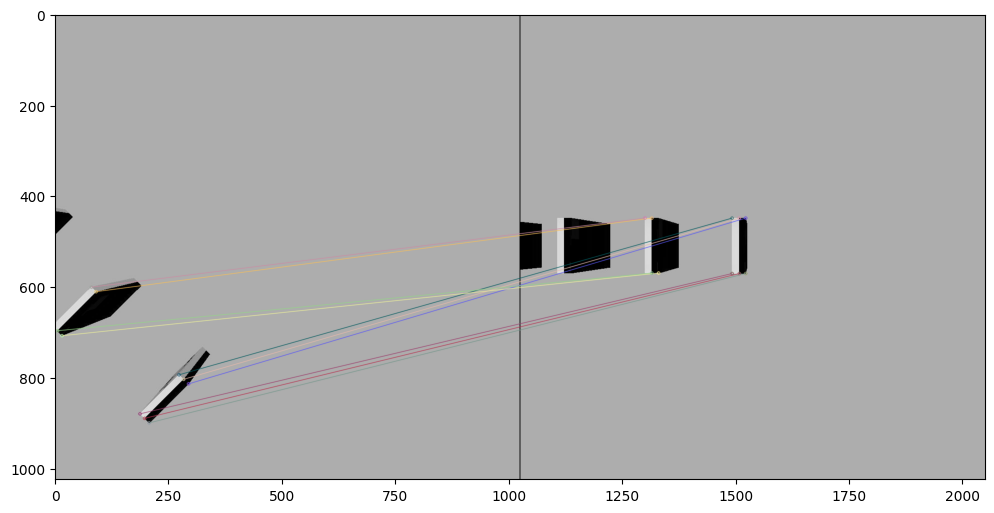
\includegraphics[width=\textwidth]{figures/matchDominoes.png}
        \caption{Domino objects}
    \end{subfigure}
    \caption{Live and demonstration images used in test suite, with human marked keypoint matches}
    \label{fig:testImages}
\end{figure}


By analysing these images we can understand why some of the objects are more sensitive to noise, as explored in \refsec{sec:noise-test}.
%TODO include observations from second test. ie which objects are forgiving, which fail more tests (i bet sphere)

\subsubsection{Lego object}
In this object the keypoints are marked as the 4 corners. It is very easy to identify these even when the object was rotated. This explains why this object had the lowest systematic error (as discussed in \refsec{sec:noise-test}) because the human error was very close to 0.

\subsubsection{Mug object}
In this object the keypoints are marked at even intervals around the mug, as well as the corners of the handle. However, in the demonstration image, the top of the mug is out of frame. This reduces how many keypoints we can identify. The circular nature of this object makes placing keypoints in the exact correct position more challenging.

\subsubsection{Ball Object}
This object is surprisingly difficult to mark keypoints given it is a perfect sphere. As such keypoints move in difficult to predict ways for a human keypoint matcher. Furthermore, the 

\subsubsection{Jenga block object}
This object experienced the largest amount of systematic error by a large margin in \refsec{sec:noise-test}. Initially one might think that it should be easy to identify keypoints. Like with the Lego object, we may try to mark the corners of the block. However, in the demonstration image the top of the block is out of frame. This is deliberate to make the test more challenging for the system. As a result we can only mark the bottom two corners as keypoints. Instead we match identifiable points of the text on the object. This allows us to manually identify far more keypoints, the most of any object at 22. However, these keypoints are prone to a large amount of human error, since the text does not form clean lines in the bitmap image. As such in the rotated live image, it can be difficult to locate the correct pixel. The human error across all the keypoints accumulates, leading to the largest systematic error of any object in the test suite.

\subsubsection{Dominoes}
This object is interesting because it is actually not a single object but multiple. The rotation applied in \reftab{tab:test-suite} is not applied about the centre like other objects. The line is rotated about the first domino. This presents some challenges for the robot since in order to knock over the domino line successfully it needs to rotate the vector it approaches at, unlike most objects where the angle of approach does not matter, provided the end effector is spun to the correct angle.\\

In this test we can only identify a small number of keypoints since the majority of the domino line is out if frame.


\chapter{Additional Evaluation Figures}
\label{apx:more-figures}

This appendix contains additional figures from the evaluation in \refchap{chap:evaluation}. These figures contain additional or alternative information which can give further insight into the conclusions drawn in that section. However, they are relegated to this appendix due to the page limit of this report, and the belief that the information displayed is less crucial than the figures included in \refchap{chap:evaluation}.\\
